% View link: https://www.overleaf.com/read/wygtrfbdkpxw#8c9d5a

\documentclass{jku-icg-thesis}

% recommended packages
\usepackage{booktabs}
\usepackage{csquotes}
\usepackage{graphicx}
\usepackage{xcolor}
\usepackage{array}
\usepackage{wrapfig}
\usepackage{tikz}
\usetikzlibrary{arrows.meta, positioning, fit}
%%\usetikzlibrary{positioning}
\usepackage{placeins}
\usepackage{subcaption}




% we recommend using biblatex for references
\usepackage[
    style=numeric,
    backend=biber, 
    ]{biblatex}

% only for blindtext (can be removed)
\usepackage{kantlipsum}

% define the title and author as usual
% the class adds a macro for the immatriculation number
\title{Glacivis}
\subtitle{An interactive tool for exploring weather data and ther influence on glaciers}
\author{Mario Viehböck}

\date{\today}

% add up to two supervisors
%    you can specify special roles like this
%       \supervisor[Erstbetreuer]{First Supervisor}
%       \supervisor[Zweitbetreuer]{Second Supervisor}
\supervisor{First Supervisor}

% provide some information on the thesis
\thesissetup{
    subject = ai,       % 'ai' or 'cs'
    study = bsc,        % 'bsc' or 'msc'
    location = Linz,
}

\addbibresource{references.bib}

%%% Copy- and searchable PDF

\input glyphtounicode
\pdfgentounicode=1

%%% Document

\begin{document}

\maketitle
	
\pagenumbering{roman}

%% Intruduction: explain the problem, data, ...
%% optional section with background info 
%% section: related work, projects from wgms, timeseries visu, gesospatial 
%% Problem characterisation ... data and tasks ... datastructures and insights
%%    what makes the data important? user tasks? 
%% solution? How does it work? naming section by tool or result ??
%%      its about to explain the task and why, not explicit how to work with it
%%      Section or Subsection abour implementation
%% section about evaluation or proove by use case 
%% future work, limitations... 
%% conclusion (compact)
%% 15 - 20 pages (main matter)
%% appendix


\ClearPage

\newgeometry{left=5cm, right=5cm}
\thispagestyle{empty}
\null\vfill

\noindent
This is a relatively short quote. An even shorter one might need adapted page margins in the \texttt{\textbackslash newgeometry} call above.
\bigskip

\begingroup
\hspace*{\fill}\itshape
\begin{tabular}{c@{~}l}
     --- A. Uthor \\
\end{tabular}
\endgroup

\vfill\vfill

\restoregeometry
\ClearPage
% !TeX spellcheck = en_GB

\chapter*{Eidesstattliche Erklärung}

Ich erkläre an Eides statt, dass ich die vorliegende Dissertation selbstständig und ohne fremde Hilfe verfasst, andere als die angegebenen Quellen und Hilfsmittel nicht benutzt bzw.~die wörtlich oder sinngemäß entnommenen Stellen als solche kenntlich gemacht habe.
%Die vorliegende Dissertation ist mit dem elektronisch übermittelten Textdokument identisch.

\vspace{3.5\baselineskip}
\signaffidavit[]
% !TeX spellcheck = en_US

\ClearPage
\pdfbookmark[1]{Abstract}{sec:abstract-en}
\chapter*{Abstract}

Data selection is one of the most important parts in every ML (Machine Learning) Task. In case of weather data, one faces a huge variety of different values with often high density. Clearly much more data than consumer hardware can process. 
Meteorologically, glaciers can be seen as a scale of climate change. By finding the most influential factors, the glacier changes might be much better predictable. Even more, our water supply in the Alps region could be better foreseen, caused by global heating. \\
In this project, one can discover ERA5 weather data by interacting with it. The conept is, to give a maximum of felxibility by keeping the interface intuitive. This gives deep insight of the data and therefore the basis, if and for what they can bes used. This is crucial for an successful ML project, safes a lot of time on model selection. Due to that, such tasks became more cost efficient and environmental friendly. 
%%% !TeX spellcheck = de_DE

\begin{otherlanguage}{ngerman}

\ClearPage
\pdfbookmark[1]{Kurzfassung}{sec:abstract-de}
\chapter*{Kurzfassung}

\kant[1]

\end{otherlanguage}
% !TeX spellcheck = en_US

\ClearPage
\pdfbookmark[1]{Acknowledgements}{sec:acknowledgements}
\chapter*{Acknowledgements}

\kant[1]
\ClearPage

\pdfbookmark[1]{Contents}{sec:toc}
\tableofcontents

%\listofequations
\ClearPage

%was set to {1}, maybe {2} is not JKU conform
\setcounter{page}{2}
\pagenumbering{arabic}

%%%%%%%%%%%%%%%%%%%%%%%%%%%%%%%%%%%%%%%%%%%%%%%%%%%%%%%%%%%%%%%%%%%%%%%%%%%%%%%%
%% 
\cleardoubleoddpage%  Make sure to start each chapter on a new odd page
\chapter{Introduction}
\label{sec:introduction}
Introduction and Motivation could be one thing....

\begin{itemize}
  \item Relation between AI and Visualization
  \item Scope of the Project
  \item Teaser for the motivation
\end{itemize}

\section{Motivation}
\label{sec:introduction:motivation}

\begin{itemize}
  \item Importance of visual inspection of data
  \item Handling of the complexity of meteorological data
  \item Reduce the environmental impact and improve the outcome by better data quality
  \item building an intuitive tool to get insights to meteo data by using glaciers as a scale
\end{itemize}


\section{Objectives and Approach}
\label{sec:introduction:objectives}


\section{Outline}
\label{sec:introduction:outline}



%% 
%%%%%%%%%%%%%%%%%%%%%%%%%%%%%%%%%%%%%%%%%%%%%%%%%%%%%%%%%%%%%%%%%%%%%%%%%%%%%%%%

\chapter{Related Work}

The ERA5 dataset is widely used in climate and cryosphere research.
Numerous glacier-related studies are based on ERA5-derived products, for example the work of Fabien Maussion and collaborators \parencite{maussion_publications}.

\begin{wrapfigure}{r}{0.65\textwidth}
  \centering
  \includegraphics[width=0.55\textwidth]{reports/Thesis Report/figures/era5_ts_global_glaciers.png}
  \caption{Temperature change at glacier locations (area-weighted) compared to the global mean \cite{maussion_publications}.}
  \label{fig:era5_ts_global_glacier}
\end{wrapfigure}

As shown in Figure~\ref{fig:era5_ts_global_glacier}, the temperature change at glacier locations is stronger than the global average.
However, these studies typically focus on static analyses, and interactive exploration of the data is usually not possible.

\par\medskip

Copernicus Climate Change Service provides as a starting point several Jupyter Notebooks, where ERA5 data can be discovered \parencite{earthdatahub_tutorials}.
The interaction for a user is very restricted and usually requires changing or adding code.

\begin{wrapfigure}{r}{0.45\textwidth}
  \centering
  \includegraphics[width=0.55\textwidth]{reports/Thesis Report/figures/german_temperature.png}
  \caption{Average temperature in Germany, October 2018 \cite{earthdatahub_tutorials}.}
  \label{fig:german_temperature}
\end{wrapfigure}

\vspace{1em}

An example visualization is shown in Figure~\ref{fig:german_temperature}.
This is grat to make the first climps on it, but not enough to decide, is the data are suitable for a potetial ML task.

\vspace{1em}

WGMS provides with the \textit{Fluctuations of Glaciers Browser} \cite{arcgis_experience_836c66d} a browser tool to discover glacier on a map.
Over 100,000 glaciers are coverd.
One can get insights about the database from this glacier measurements.
But whats not possible, is to interact with measurements or directly compare them.
What is missing is an interactive tool to gain insights into ERA5 weather data and WGMS glacier data.


\vspace{1em}


\begin{figure}[htbp]
  \centering
  \includegraphics[width=0.70\textwidth]{reports/Thesis Report/figures/dachstein_glacier.png}
  \caption{Dachstein glaciers visualized via the \textit{Fluctuations of Glaciers Browser} \cite{arcgis_experience_836c66d}.}
  \label{fig:dachstein_glacier}
\end{figure}

\vspace{1em}


\begin{figure}[htbp]
  \centering
  \includegraphics[width=0.2\textwidth]{reports/Thesis Report/figures/surface_temp_berlin.png}
  \caption{Temperature development over time in Berlin \cite{earthdatahub_tutorials}.}
  \label{fig:surface_temp_berlin}
\end{figure}
\chapter{Visualization}

The objective is to create a interactive tool as a web-interface, with that a person can intuitively gain insights to the data. The project from the Seminar in AI already gives some learning's, which are the stating point of this work.

\vspace{1em}
\textbf{The concept consists of the following parts:}

\begin{itemize}
    \item Set conceptual design choices
    \item Collecting ERA5 and glacier data
    \item Data preprocessing
    \item Setup the framework of the visualization
    \item Implement one element / function after another
\end{itemize}


\section{Conceptual design choices}
\label{sec:conceptual_design_choices}

Goal is to find the optimal tradeoff between a maximum of interactivity and a intuative interface. For this, the user interface is seperated into 4 sections.

\begin{figure}[htbp]
\centering
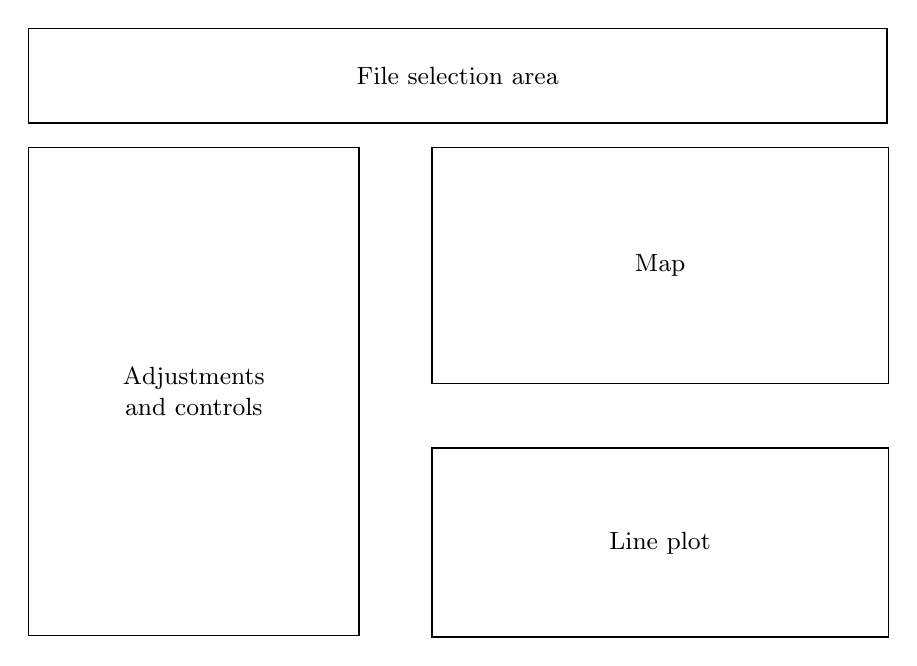
\begin{tikzpicture}[
  box/.style={draw, line width=0.6pt, align=center, minimum height=1.2cm},
  smallbox/.style={box, minimum width=5.8cm},
  tallbox/.style={box, minimum width=4.2cm, minimum height=6.2cm},
  widebox/.style={box, minimum width=10.9cm},
  font=\small
]

% Top: file selection
\node[widebox] (top) {File selection area};

% Left: controls
\node[tallbox, below=0.9cm of top.west, anchor=north west] (ctrl) {Adjustments\\and controls};

% Right: map + line plot
\node[smallbox, right=0.9cm of ctrl.north east, anchor=north west, minimum height=3.0cm] (map) {Map};
\node[smallbox, below=0.8cm of map, minimum height=2.4cm] (plot) {Line plot};

\end{tikzpicture}
\caption{Conceptual layout of the user interface, showing the separation of data selection, parameter controls, and visualization views.}
\label{fig:ui_layout}
\end{figure}

The workflow is starting from the top-left and ends on the bottom-right. Like when reading a book. This should provide the basic structure for an intuitive handling.
Of course, in all sections, interaction will be possible. But they will influence each other only top-down:
\textbf{File selection} $\rightarrow$ \textbf{Adjustments and controls} $\rightarrow$ \textbf{Map} $\rightarrow$ \textbf{Line Plot}


\section{Data Preprocessing}

ECMWF provides ERA5 data in GRIB\cite{ecmwf_grib_explanation} format. The GRIB format is designed to storing data and distribute them. There are Python libraries, which can read this format but for the visualisation task in this project, GRIB-files are not ideal.

According to \textcite[pp.~85--87]{python_maps}, the library \textit{Xarray} is optimized for performing labeled multi-dimensional computations and subsequent visualization of geospatial data. 
Working directly with GRIB files, however, can create a computational bottleneck in this environment due to their structure and decoding requirements. 
Both \textit{Python Maps} \parencite[p.~88]{python_maps} and the official Xarray documentation \parencite{xarray_documentation} recommend the use of the NetCDF format for efficient storage and processing of scientific data. 
NetCDF provides a self-describing and platform-independent data model that is particularly well suited for climate and meteorological datasets \parencite{netcdf_documentation}.




\begin{figure}[htbp]
\centering
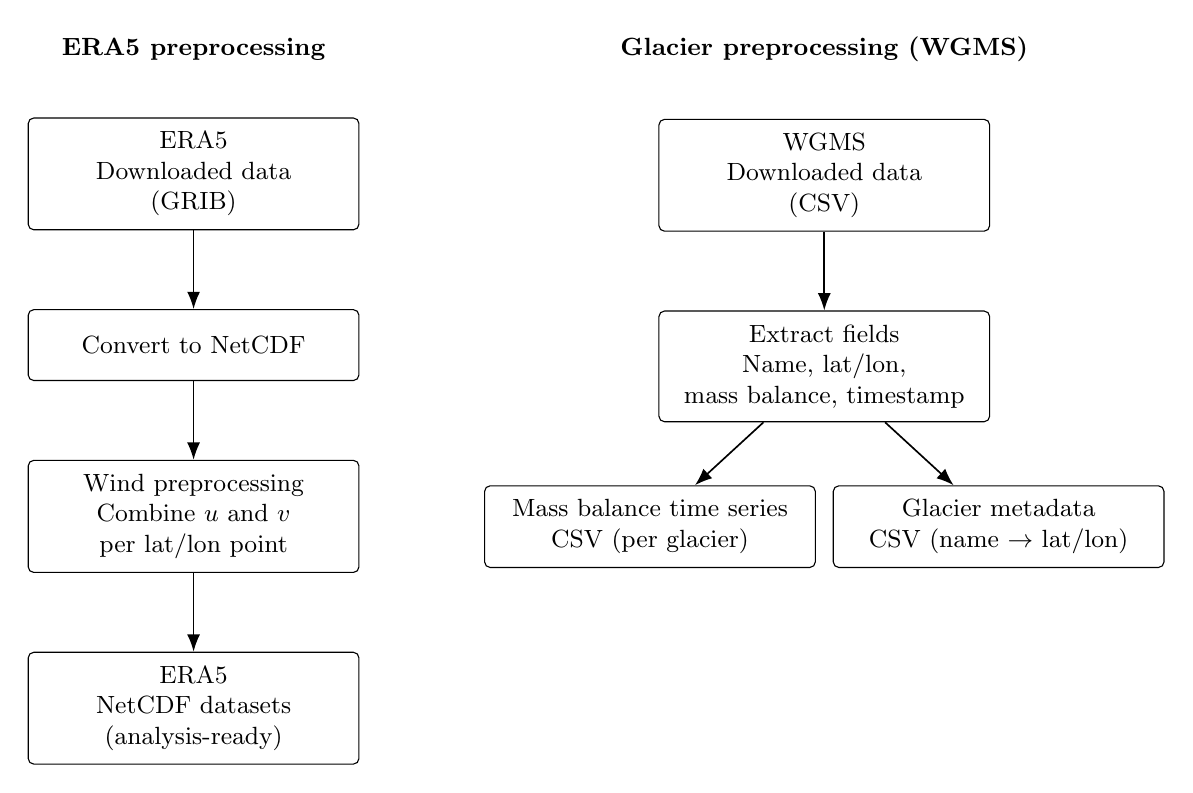
\begin{tikzpicture}[
  font=\small,
  node distance=10mm and 10mm,
  box/.style={
    draw,
    rounded corners=2pt,
    align=center,
    inner sep=5pt,
    minimum height=9mm,
    minimum width=42mm
  },
  arrow/.style={-{Latex[length=2.2mm]}, line width=0.6pt}
]

% ================= ERA5 branch =================
\node[font=\small\bfseries] (era5_title) {ERA5 preprocessing};

\node[box, below=6mm of era5_title] (era5_raw)
  {ERA5\\Downloaded data\\(GRIB)};

\node[box, below=of era5_raw] (era5_conv)
  {Convert to NetCDF};

\node[box, below=of era5_conv] (era5_wind)
  {Wind preprocessing\\Combine $u$ and $v$\\per lat/lon point};

\node[box, below=of era5_wind] (era5_out)
  {ERA5\\NetCDF datasets\\(analysis-ready)};

\draw[arrow] (era5_raw) -- (era5_conv);
\draw[arrow] (era5_conv) -- (era5_wind);
\draw[arrow] (era5_wind) -- (era5_out);

% ================= WGMS branch =================
\node[font=\small\bfseries, right=35mm of era5_title] (wgms_title)
  {Glacier preprocessing (WGMS)};

\node[box, below=6mm of wgms_title] (wgms_raw)
  {WGMS\\Downloaded data\\(CSV)};

\node[box, below=of wgms_raw] (wgms_extract)
  {Extract fields\\Name, lat/lon,\\mass balance, timestamp};

% Parallel outputs (tighter spacing)
\node[box, below left=8mm and -20mm of wgms_extract] (wgms_mass)
  {Mass balance time series\\CSV (per glacier)};

\node[box, below right=8mm and -20mm of wgms_extract] (wgms_meta)
  {Glacier metadata\\CSV (name $\rightarrow$ lat/lon)};


\draw[arrow] (wgms_raw) -- (wgms_extract);
\draw[arrow] (wgms_extract) -- (wgms_mass);
\draw[arrow] (wgms_extract) -- (wgms_meta);

\end{tikzpicture}
\caption{Data preprocessing workflow for ERA5 meteorological data and WGMS glacier data.}
\label{fig:data_preprocessing_workflow}
\end{figure}




\newpage


\section{User Interface}

-- Parts and interaction, design choice 

\subsection{Environment and packages}
With the learning's from the Seminar in AI project and some trial and error, the following approach seems to be optimal: \textit{Panel} as framework for the web interface + \textit{Bokeh} for the visualization and interaction elements.

\vspace{1em}
\textbf{Panel}

Panel is an open-source Python library designed to streamline the development of robust tools, dashboards, and complex applications entirely within Python. With a comprehensive philosophy, Panel integrates seamlessly with the PyData ecosystem, offering powerful, interactive data tables, visualizations, and much more, to unlock, visualize, share, and collaborate on your data for efficient workflows.

Its feature set includes high-level reactive APIs and lower-level callback-based APIs, enabling rapid development of exploratory applications and facilitating the creation of intricate, multi-page applications with extensive interactivity.

Panel is a proud member of the HoloViz ecosystem, providing a gateway to a cohesive suite of data exploration tools.

\vspace{1em}
\textbf{Bokeh}

Bokeh is a Python library for creating interactive visualizations for modern web browsers. It helps you build beautiful graphics, ranging from simple plots to complex dashboards with streaming datasets. With Bokeh, you can create JavaScript-powered visualizations without writing any JavaScript yourself.

\vspace{1em}

As in Conceptual design choices,\ref{sec:conceptual_design_choices}, the user interface is separated into 4 sections. 

\subsection{File selection}

Follow the intuitive left-to-right approach.

\begin{figure}[htbp]
  \centering
  \includegraphics[width=1.05\textwidth]{reports/Thesis Report/figures/interface_file_selection.png}
  \caption{File selection field with the slider for pre filtering the time range.}
  \label{fig:interface_file_selection}
\end{figure}


\newpage
\subsection{Adjustments and Controls}

Compromise between clean structure and a maximum of freedom.


\begin{wrapfigure}{r}{0.7\textwidth}
  \centering
  \includegraphics[width=0.6\textwidth]{reports/Thesis Report/figures/interface_controls.png}
  \caption{Area of controls, which are influences all upcoming visualizations}
  \label{fig:interface_controls}
\end{wrapfigure}

text text



\newpage



\FloatBarrier

\subsection{Map}


\begin{figure}[htbp]
  \centering

  \begin{subfigure}{0.49\textwidth}
    \centering
    \includegraphics[width=\linewidth]{reports/Thesis Report/figures/interface_map_temperature.png}
    \caption{Map with temperature.}
    \label{fig:interface_map_temperature}
  \end{subfigure}
  \hfill
  \begin{subfigure}{0.49\textwidth}
    \centering
    \includegraphics[width=\linewidth]{reports/Thesis Report/figures/interface_map_wind.png}
    \caption{Map with wind.}
    \label{fig:interface_map_wind}
  \end{subfigure}

  \caption{Comparison of the map visualization using different meteorological variables.}
  \label{fig:interface_map_comparison}
\end{figure}



\subsection{Timeseries plot}

Line plot, 2 in Wind mode. 

\begin{figure}[htbp]
  \centering
  \includegraphics[width=1.05\textwidth]{reports/Thesis Report/figures/interface_line_plot.png}
  \caption{lineplot with temperature}
  \label{fig:interface_line_plot}
\end{figure}


And with glacier data:


sample textsample textsample text
sample textsample text
sample text





\begin{figure}[htbp]
  \centering
  \includegraphics[width=1.05\textwidth]{reports/Thesis Report/figures/interface_line_plot_wind.png}
  \caption{lineplot with wind}
  \label{fig:interface_line_plot_wind}
\end{figure}





\newpage


\section{Implementation}

Here I want to provide some insights, how the implementation is done. I will focus only on the key parts and the most important learnings.

Panel + Bokeh




\chapter{Use Case}

\section{Hypothesis}

Wind speed and direction changed over the years, to a stronger wind from south. This significantly influences the glacier melt. \\

This hypothesis is based on the assumption that due to general higher temperatures, the atmospheric pressure over the Mediterranean Sea increases on average, compared to the Northern Alps region. And as a result, more south Foehn days are seen over the main ridge, which causes temporarily high temperatures in affected areas.

\section{Proof with glaciVis}

walk-through 
\chapter{discussion}

For temperature data and even more for wind data from ERA5, this tools can provide very useful insights. The low computational effort combined with the easy to use interface makes it absolute useful.
At the beginning of this project, a scope was set up to focus on keypoints due to natural time constraints. Now we can take a look into reasonably limitations and practical next steps.


\section{Limitations}

\paragraph{Variables from ERA5}
Given that ERA5-Land consists of 49 variables, the implemented two variables can only represent a starting point.

\paragraph{WGMS data}
For the glaciers, only mass balance is considered. Including additional parameters, such as glacier area, could provide further insights. However, this would require a deeper understanding of glacier-specific data structures in order to ensure comparability.

\paragraph{Statistical tools}
Currently, a user can choose one of 4 trend line methods. Also mean, minimum, maximum and the number of the selected data points are provided. For deeper investigation, more advanced statistical methods might be beneficial. 

\paragraph{Data loading}
ERA5 data must be downloaded from Copernicus Climate Data Store (CDS)\parencite{era5_single_levels}. This can be done either by selecting the data of choice via web interface and download as a batch in ZIP format or by using an API. However, the amount of data (batch size) is limited. It also can take hours, if the batch size is towards to the allowed limit. So this is an inherent limitation from the data source about data-fetching. This needs to taken into account 



\section{future work}

Hence the tools showed its usability in deeply discovering weather data from ERA5, there is also the biggest potential of improvements.

\paragraph{Adding variables}
Implement more variables like \textit{Snowfall}, \textit{Snow depth} and \textit{Snow density} are the next logical step. Changes in the realtion of this three values can be potential features for a predation task.

\paragraph{Combination of ERA5 datasets}
More advanced but very interesting would be the implemetation of values on several levels. For example the dataset \textit{ERA5 hourly data on pressure levels} provides variables like \textit{Fraction of cloud cover} and \textit{Temperature} on 19 atmospheric pressure levels. 
\chapter{conclusion}

The very first idea to visually compare glacier data and meteorological data in some kind of plot, does work just partly.
One reason for that is the different nature of glacier observations and reanalyzed ERA5 data. Even reference glaciers are measured/claculated there changes once a year. Few years ago, not even that.

During the developent process, it turns out, this tool is surpringsingly well suited to get deep insights into meteorological data. So one can precisely decide, if a dataset is suitable for some task. And if yes, which resolution in time and which area is necessary.



\listoffigures
\listoftables


\printbibliography[title = {References}, heading = bibintoc]

\begin{icgAppendix}
  \include{ax-appendix}
\end{icgAppendix}

\end{document}
